\section{Mixer}\label{mixer}

Mixer

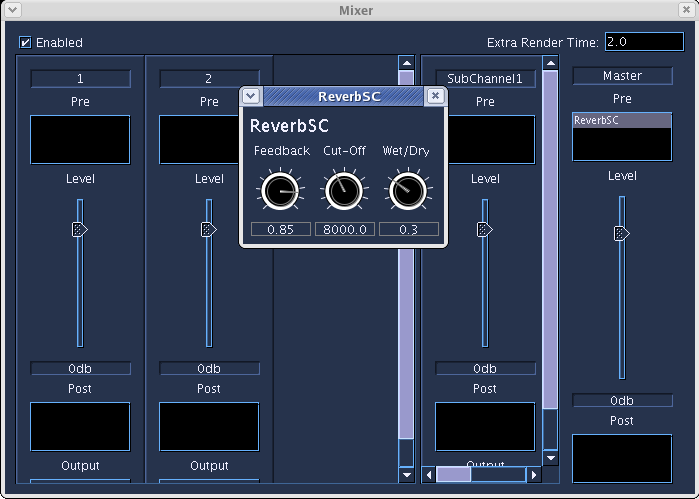
\includegraphics{images/mixer.png}

The Mixer system in blue allows for graphically editing levels for
instruments, applying pre- and post-fader effects, and routing and
mixing of signals through subchannels.

\subsection{Architecture}

The Mixer system has three panel sections:

\begin{description}
\item[Channels]
Channels are auto-created and bound to Instrument ID's in the Orchestra
for a Project. In the Mixer Dialog they are located in the first section
on the left within a splitpane that separates them from the SubChannels.
Channels can be set to route to either SubChannels or directly to the
Master Channel.
\item[SubChannels]
SubChannels are user-created and are located in the center section of
the Mixer Dialog, on the right side of the splitpane. Channels can be
set to route to SubChannels, and SubChannels can route into other
SubChannels or out to the Master Channel.
\item[Master Channel]
The Master Channel is located on the right side of the Mixer Dialog.
There is only one master Channel per project which all channel and
subchannel signals ultimately route through.
\end{description}

Each channel allows for applying effects to the incoming signal either
pre- or post-fader.

\subsection{Using the Mixer}

For most MIDI-based music composition environments, the typical user
interaction with a Mixer system is that users first create tracks on a
timeline, and for each track an audio channel is automatically bound in
the mixer. The user then selects an instrument for that track(if it is a
MIDI track); MIDI information from the track is routed to the instrument
and that instrument generates audio signals. If the instrument happens
to be a software synthesizer, the audio signals are then usually taken
from the instrument and routed out to the Mixer channel that has been
bound to that track.

However, since blue does not bind music information on a SoundLayer to
an instrument (you can have heterogenous note data generated in any
soundObject for any number of instruments, a flexibility which allows
for soundObjects to be more representative of musical ideas), and nor
does it bind SoundLayers to channels, the abstraction of the musical
system and the interaction with the Mixer system requires different
handling.

In blue's Mixer system, Mixer channels are automatically bound to
instruments by their instrument ID. Binding to ID and not per-instrument
in the Orchestra allows for the case where users have set multiple
instruments to the same instrument ID but only having one which is
enabled. If you then disable one and then enable another instrument to
test out different instruments with the same musical note data, the
mixer channel's settings will be maintained for the new instrument as it
is bound by ID.

Channels in themselves can not be created or removed directly by the
user, but are automatically added or removed depending on how how
instruments are added and removed from the project's orchestra. For
cases of when an instrument has an ID and a user wishes to change the
ID, if the new ID already exists and a channel is already created, the
old channel is removed as long as no other instrument has the old ID. If
the new channel ID has no existing mixer channel bound to it and if the
channel for the old ID only has one instrument with that ID (the
instrument that is changing ID's), the bound mixer channel is simply
reassigned to the new ID and maintains its settings.

Subchannels are added by right-clicking with in the SubChannels area and
choosing "Add SubChannel" from the popup menu. To remove a subchannel
right-click the channel strip to be removed and select "Remove" from the
popup menu.

At the bottom of every Channel and SubChannel strip is an output
dropdown box to choose where to route that Chanel's audio to. For
SubChannels, they can only route to other SubChannels which lead to the
Master Channel, meaning that there is no feedback allowed (i.e. routing
SubChannelA to SubChannelB and then to SubChannelC and that back to
SubChannelA is not allowed as it would create a loop).

For the instruments in the orchestra to be able to route out to the
Mixer, a special pseudo-opcode must be used for the output of the
instrument, entitled "blueMixerOut". You use blueMixerOut in the same
way as the outc opcode. If the Mixer is not enabled in the Dialog, when
blue goes to process the instrument, blueMixerOut will be replaced with
outc, thus making the audio of that instrument directly route out to dac
or disk, depending on how Csound is set to render. If the Mixer is
enabled, blueMixerOut is translated into global variables and the
Mixer's instrument code is generated automatically without the user
having to worry about the code details of setting up a Mixer system
themselves in Csound code.

There is also a subChannel form of blueMixerOut available that is able
to target a subchannel by name. This form is used in the following way:

\begin{verbatim}
      blueMixerOut "subChannelName", asig1, asig2 [, asig3...]
    
\end{verbatim}

Using this form, the asig signals will be mixed into the subChannel
given by name. This form is available to use within Instruments but is
also very useful to use when working Sound SoundObjects and AudioFile
SoundObjects, which do not have channels created for them. This way, you
can route the output of an AudioFile to a named subchannel and apply
Effects, etc.

\subsection{Effects}

Effects in blue are implemented as User-Defined Opcodes, and
understanding of how User-Defined Opcodes work in Csound is recommended
before creating Effects. Understanding how UDO's work however is not
necessary if one simply wants to use Effects.

The workflow for using Effects with your Mixer channels is:

\begin{enumerate}
\def\labelenumi{\arabic{enumi}.}
\item
  Populate your Effects Library by either creating effects or importing
  them from blueShare.
\item
  In the Mixer, choose either the pre-fader or post-fader effects bin to
  add effects. Right click on the bins to open up a popup menu that
  shows effects that are currently in your library from which to choose
  to insert.
\item
  In the Mixer, choose either the pre-fader or post-fader effects bin to
  add effects. Right click on the bins to open up a popup menu that
  shows effects that are currently in your library from which to choose
  to insert.
\item
  Configure your effect by double-clicking it in the effects bin.
  Double-clicking the effect will open up a dialog that shows the
  effect's graphical user interface.
\end{enumerate}

Effects Library

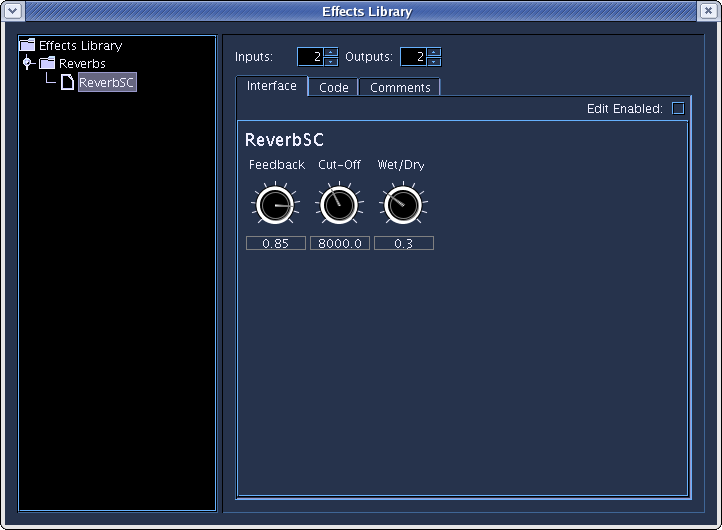
\includegraphics{images/effectsLibrary1.png}

Effects are created and managed in your Effects Library, which is
accessible from the Tools menu. The Effects Library is program wide, so
any Effect in the library will be accessible to use from any project you
are working on.

In the picture above, you will see the library where one can create
Effects as well as organize them into groups. The organization into
groups within the library will be reflected in the Effects popup that
appears when the user is looking to add Effects to their Mixer channels.

To add a group or new Effect, right click on any node and choose the
option from the popup. The popup will also allow you to cut/copy/paste
groups or Effects which is useful when reorganizing or when creating new
Effects based on older ones.

Once an Effect or group is added, you can edit the the name by
double-clicking the node in the tree. Selecting an effect by clicking it
once will populate the editor on the right. The picture above shows the
User Interface editor for the Effect. Like other BlueSynthBuilder-based
editors in blue, clicking Edit Enabled will allow you to move between to
edit modes, one in which you can add, remove, and move around widgets,
and another where you can interact with the widgets (useful for setting
an initial value for the Effect.)

Effects Library

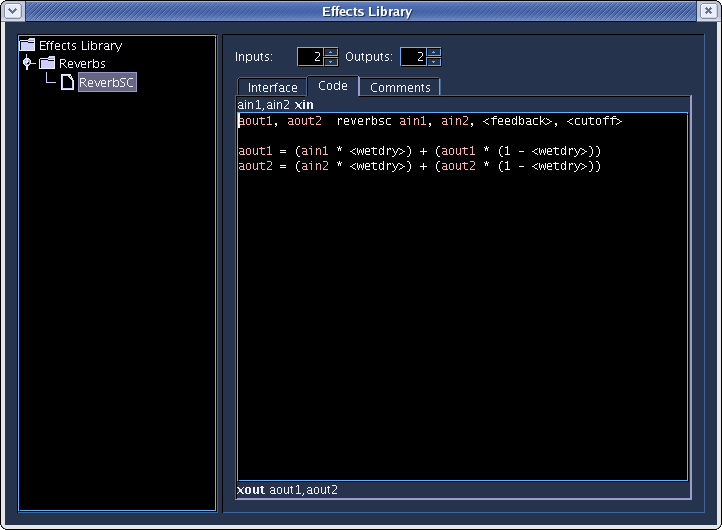
\includegraphics{images/effectsLibrary2.png}

In the code editor for the Effect, one sees that the xin and xout lines
of the User-Defined opcode display according the number of in and out
audio signals the Effect will support. The names of the signals are
hard-coded, which makes it easier for others to know exactly what the
incoming and outgoing signals will be should they look at your code.

Code for the Effect should follow the same principles as User-Defined
Opcodes(i.e. one can add a setksmps line at the top of the code area).
Values from the widgets follow the same principles as BlueSynthBuilder,
and code completion for opcodes (ctrl-space) and BSB widgets
(ctrl-shift-space) work within the code editor.

\begin{quote}
\textbf{Note}

blue currently expects Effects to have nchnls number of channels in and
out where nchnls is the number set by the project.
\end{quote}

\subsection{Other Notes}

\begin{itemize}
\item
  The Extra Render Time option in the Mixer dialog allows the user to
  add extra time to the end of the score. This is useful to allow time
  for Effects which may have time delay (i.e. 3-second long reverb) to
  have time enough for processing, as well as simply to add time at the
  end of a piece.
\end{itemize}

\subsection{Sends}

Besides effects, users are also able to put in Sends into the pre- and
post-fader Effects bins. Sends will output the signal from that point in
the channel's signal chain to a selected SubChannel. As with the output
channels, Sends can only feed-forward down the chain to the Master Out
and can not be made to create a feedback loop. Users are able to set the
channel to send to as well as the amount to send. This send amount is
also able to be Automated, just as the Effects are.

\subsection{Randomization}

Widget values are able to be randomized in the same way as in the
BlueSynthBuilder, and is available in the usage mode when working with
Effects in the Effects Library or when using Effects from the mixer.
Please further information, please see the documentation for
\protect\hyperlink{bsbWidgetRandomization}{BlueSynthBuilder Widget
Randomization}.

\subsection{Code Generation Optimization}

blue's mixer system optimizes when generated code for Csound to use.
When compiling down to ORC code, blue checks all signal paths to see if
any path will result in unused audio and if so, will optimize out any
code that is along that path. The rules for optimization are as follows:

\begin{itemize}
\item
  If channel does not generate signal to channel output (if no
  automation for level fader and fader == -96.0f), only generate code up
  to last send in preFader effects chain
\item
  When processing Sends, checks down the graph to see if send signal
  will make it to the Master output or not, checking both down graph of
  output channels as well as sends for each channel. If not, does not
  generate output for Send.
\item
  If channel does not have channel output and no valid prefader sends,
  do not generate anything for channel.
\item
  If SubChannel has no signal inputs (whether it's from another
  Channel's out channel, a Send, or dependency from code that uses the
  subChannel form of blueMixerOut), do not generate anything for
  channel.
\end{itemize}
